\documentclass[a4paper]{article}

%% Language and font encodings
\usepackage[english]{babel}
\usepackage[utf8x]{inputenc}
\usepackage[T1]{fontenc}


% From https://gist.github.com/timvdalen/3796300
% From https://hackage.haskell.org/package/alloy-1.2.0/src/tutorial/tutorial.tex
\usepackage{color}
\usepackage{listings} % For Alloy code highlights
% alloy.sty
% Alloy mode for the LaTeX listings package.
% This is public domain

\lstdefinelanguage{alloy}{
  keywords={%
      assert, pred, all, no, lone, one, some, check, run,
      but, let, implies, not, iff, in, and, or, set, sig, Int, int,
      if, then, else, exactly, disj, fact, fun, module, abstract,
      extends, open, none, univ, iden, seq,
  },
  literate=%
    %{:}{$\colon$}1
    %{|}{$\bullet$}1
    %{==}{$=$}1
    %{=}{$=$}1
    %{!=}{$\neq$}1
    %{&&}{$\land$}1
    %{||}{$\lor$}1
    %{<=}{$\le$}1
    %{>=}{$\ge$}1
    %{all}{$\forall$}1
    %{exists}{$\exists$}1
    %{!in}{$\not\in$}1
    %{\\in}{$\in$}1
    %{=>}{$\implies$}2
    % the following isn't actually Alloy, but it gives the option to produce nicer latex
    {|=>}{$\Rightarrow$}2
    {<=set}{$\subseteq$}1
    {+set}{$\cup$}1
    {*set}{$\cap$}1
    {==>}{$\Longrightarrow$}3
    {<==>}{$\Longleftrightarrow$}4
    {...}{$\ldots$}1
    {\\hl}{$\hline$}1
    {\\alpha}{$\alpha$}1
    {\\beta}{$\beta$}1
    {\\gamma}{$\gamma$}1
    {\\delta}{$\delta$}1
    {\\epsilon}{$\epsilon$}1
    {\\zeta}{$\zeta$}1
    {\\eta}{$\eta$}1
    {\\theta}{$\theta$}1
    {\\iota}{$\iota$}1
    {\\kappa}{$\kappa$}1
    {\\lambda}{$\lambda$}1
    {\\mu}{$\mu$}1
    {\\nu}{$\nu$}1
    {\\xi}{$\xi$}1
    {\\pi}{$\pi$}1
    {\\rho}{$\rho$}1
    {\\sigma}{$\sigma$}1
    {\\tau}{$\tau$}1
    {\\upsilon}{$\upsilon$}1
    {\\phi}{$\phi$}1
    {\\chi}{$\chi$}1
    {\\psi}{$\psi$}1
    {\\omega}{$\omega$}1
    {\\Gamma}{$\Gamma$}1
    {\\Delta}{$\Delta$}1
    {\\Theta}{$\Theta$}1
    {\\Lambda}{$\Lambda$}1
    {\\Xi}{$\Xi$}1
    {\\Pi}{$\Pi$}1
    {\\Sigma}{$\Sigma$}1
    {\\Upsilon}{$\Upsilon$}1
    {\\Phi}{$\Phi$}1
    {\\Psi}{$\Psi$}1
    {\\Omega}{$\Omega$}1
    {\\EOF}{\;}1
    ,
  sensitive=true,  % case sensitive
  morecomment=[l]//,%
  morecomment=[l]{--},%
  morecomment=[s]{/*}{*/},%
  morestring=[b]",
  numbers=none,
  firstnumber=1,
  numberstyle=\tiny,
  stepnumber=2,
  basicstyle=\scriptsize\ttfamily,
  commentstyle=\itshape,
  keywordstyle=\bfseries,
  ndkeywordstyle=\bfseries,
}

\lstset{ % General setup for the package
	language=alloy,
	basicstyle=\normalsize\sffamily,
	%numbers=left,
    %backgroundcolor=\color{lightgray},
 	%numberstyle=\tiny,
	%frame=tb,
	tabsize=4,
	columns=fixed,
	%showstringspaces=false,
	%showtabs=false,
	keepspaces,
	commentstyle=\color{green}, %#157415
	keywordstyle=\color{blue} %#191978
}
% End of Alloy highlights

%% Sets page size and margins
\usepackage[a4paper,top=3cm,bottom=2cm,left=3cm,right=3cm,marginparwidth=1.75cm]{geometry}

%% Useful packages
\usepackage{amsmath}
\usepackage{graphicx}
\usepackage{verbatim}
\usepackage[colorinlistoftodos]{todonotes}
\usepackage[colorlinks=true, allcolors=black]{hyperref}

\title{Requirements Analysis and Specifications Document}
\author{Software Engineering 2}
\date{November 13,2016}

\begin{document}
\maketitle

\begin{figure}[h]
  \centering
  
\includegraphics[width=300 pt]{resources/polimi.png}
  \label{fig:polimi}
\end{figure}

\emph{\\}
\emph{\\}
\emph{\\}
\emph{\\}
\emph{\\}
\emph{\\}
\emph{\\}
\emph{\\}
\emph{\\}
\emph{\\}

\begin{minipage}{0.7\textwidth}
\begin{flushleft} \large
\emph{Authors:}\\
Claudio Salvatore \textsc{Arcidiacono} Matr 879109\\
Antonio \emph{ }\emph{ }\emph{ }\emph{ }\emph{ }\emph{ }\emph{ }\emph{ }\emph{ }\emph{ }\emph{ }\emph{ }\textsc{Di Bello} \emph{ }\emph{ }\emph{ }\emph{ } Matr 878786\\
Denis  \emph{ }\emph{ }\emph{ }\emph{ }\emph{ }\emph{ }\emph{ }\emph{ }\emph{ }\emph{ }\emph{ }\emph{ }\emph{ }\emph{ }\emph{ }\textsc{Dushi } \emph{ }\emph{ }\emph{ }\emph{ }\emph{ }\emph{ }\emph{ }\emph{ }\emph{ }Matr 879115
\end{flushleft}
\end{minipage}

\begin{minipage}{0.4\textwidth}

\end{minipage}

\pagenumbering{gobble}
\newpage
\pagenumbering{arabic}

\tableofcontents

\newpage

\section{Introduction}

\subsection{Description of the given problem}
We will project and implement PowerEnJoy, which is a digital management system for a car-sharing service that exclusively employs electric cars.
The system that will be developed has to allow users to register and log in to the service, to see which car are available and were the cars can be parked. In addition to the basic functionality of a car-sharing service the system has to incentive virtuous behaviors of the users, like plugging the car to a charging station or leaving the car with enough charge, in order to have as much as possible a self-sustainable service.

\subsection{Goals}

\begin{itemize}
\item [G1]A client can register to the system by providing an e-mail, valid payment information and a photo of his driving license.

\item [G2]A client can log in to system.

\item [G3]Allows clients to obtain information about available cars(position and remaining charge), safe areas(boundaries) and charging stations (position and available plugs).

\item [G4]Allows clients to reserve a car that fits most their needs.

\item [G5]A client can start the rent opening a car that has reserved previously when he/she is in the near by.

\item [G6]During the rent a client can display the amount of money charged.

\item [G7]Guarantee as many available cars as possible encouraging clients to have a virtuous and eco-friendly behavior applying fees and discounts.

\item [G8]Allows clients to end the rent and leave the car in any safe area.

\item [G9]Clients can report eventual damages made by users that have driven the car before.

\item [G10]Clients can set the money saving option.


\end{itemize}


\subsection{Domain assumption}
We suppose that these properties hold in the analyzed world :
\begin{itemize}
\item All cars have a stable GPS signal.
\item Clients shares their position when they use the application.
\item PowerEnJoy always has updated data about all the cars and the power stations.
\item The power grid always guarantees electric power.
\item The only method to enter in a car is by the doors.
\item The company cars have at least 4 seats.
\item The streets are correctly mapped in the system.
\item All cars have stable internet connection.
\item The charging sensor reflects the real charge of the car in real-time.
\item The real charge of parked cars stays the same over time. 
\item Charging stations are not in the same GPS position.
\item There aren't two clients with the same  personal data.
\end{itemize}

\newpage

\subsection{Glossary}
\textbf{Guest:}
 is an user that is not registered yet to PowerEnJoy.\\
\textbf{Client:}
is an user that has completed successfully the registration procedure.\\
\textbf{Logged client:}
is a client that has logged into PowerEnJoy.\\
\textbf{Blocked client:}
is a client that is not allowed to log in to system because he has some debits with PowerEnJoy.\\
\textbf{User:}
a client or a guest.\\
\textbf{Virtuous  behavior:}
the client has a "Virtuous behavior" if he performs one or more of the following actions: 
\begin{itemize}
\item transport at least other two passengers into the car.
\item leaves the car with less than 50\% of the battery empty.
\item plugs the car into the power grid of a charging station.
\end{itemize}
\emph{\\}
\textbf{Rent:} defines the period of time that starts when the logged client opens the car and ends when the door of the car are locked due to a "end rent" request of the logged client.\\
\textbf{Pin:} a personal sequence of four numbers given by the system after the registration, necessary to start the engine.\\
\textbf{Map Information:}
denotes the following information: 
\begin{itemize}
\item location of available cars.
\item location of charging areas.
\item for each charging area the number of available charging spots.
\item boundaries of safe areas.
\end{itemize}
\emph{\\}
\textbf{Not valid data:}
syntactically incorrect data (e.g. mail not in the format local-part@domain).\\
\textbf{Credentials:}
email and password used to log into PowerEnJoy.\\
\textbf{Valid Credentials:}
email and password related to a registered user.\\
\textbf{Car information Menu:}
displayed when a client selects a car on the map. In this menu are displayed the information about the car (remaining charge percentage and license plate number) and a button that can be used to reserve the car.\\
\textbf{Safe Areas:} 
areas in which is permitted to the client to end the rent and leave the car.\\
\textbf{Valid Payment Information:}Credit or prepaid card with at least a minimum amount of money.\\

\subsection{Synonymous}
\begin{itemize}
\item rental: rent 
\item charging area: charging station
\item client : logged client. Sometimes an action can be performed only by a client that has logged previously. We will use client instead of logged client when this distinction is not ambiguous.
\end{itemize}

\subsection{Interfaces to external applications}
The PowerEnJoy system interacts with the following external systems:
\begin{itemize}
\item \textbf{Operators system:} to share with operators information about the rental chronology, the cars position, remaining charge and  reports of damaged/dirty car for maintenance and legal purposes. 
\item  \textbf{Civil registry office:} to obtain user profile information from ID number.
\item \textbf{Transport authority:}  to obtain user profile information from license number.
\item \textbf{Payment gateway:} to verify the validity of the payment information and to charge the clients. 
\end{itemize}


\subsection{Reference Documents}
\begin{itemize}
\item Specification Document: Assignments AA 2016-2017.pdf
\item  IEEE Std 830-1998 IEEE Recommended Practice for Software Requirements
Specifications.
\item  Examples documents:  
\begin{itemize}
\item MeteoCal RASD example2.pdf
\item RASD sample from Oct. 20lecture.pdf 
\end {itemize}
\end {itemize}

\newpage

\section{Actors}
\begin{itemize}
\item \textbf{Guest:} this user hasn't registered to PowerEnJoy yet but he is allowed to view the map with all the information in the website or in the mobile application. To access to other functionality, like reservation, this type of user has to complete the registration procedure.

\item \textbf{Client:} A Guest that performs correctly a registration procedure becomes a Client. The Client can log in to the PowerEnJoy platform using the e-mail provided during registration and password provided by system.

\item \textbf{Logged Client:} Once the Client has logged into PowerEnJoy platform he is considered as a Logged Client. A Logged Client can still view the map but he can also reserve a car, open the reserved car, start and end the rent. During the rent he has the possibility to report a damaged or dirty car and to select the "money saving" option. 
\end{itemize}

\newpage

\section{Requirements}
\subsection{Functional requirement}
\begin{enumerate}
\item A client can register to the system by providing an e-mail, valid payment information and a photo of his driving license.
\begin{enumerate}
\item The system must be able to check the validity of the payment information.
\item The system must be able to check if the uploaded documents are in the accepted format.
\item The system must be able to communicate with the civil registry office and transport authority in order to obtain user profile information from ID number and license number. 
\item The system must allow the registration only if ID ,license and personal information are related to the same person.
\item The system must implement a retrieve password mechanism.
\item The system should not allow to complete the registration process to an already registered user.
\item The system should not allow different users to register with the same email.
\end{enumerate}

\item A client can log in into system.
\begin{enumerate}
\item The system should provide the log in function both in the app and the web application.
\item The system should allow to rent a car only after the log in.
\item The system must guarantee that none can access to a user profile without the right credentials.
\item The system must be able to check if the credentials inserted by the user are correct.
\item The system must deny the access to blocked users.
\end{enumerate}

\item Allows clients to obtain information about
the position of available cars(position and remaining charge), safe areas(boundaries) and charging stations (position and available plugs).
\begin{enumerate}
\item The system should acquire the GPS position of available cars.
\item The system must offer a view of a map in which are displayed the position the available cars and the charging stations and the boundaries of the safe areas.
\item The system should update in real time the information about the charging stations and available cars.
\item The system must detect the position of clients that have opened the application.
\end{enumerate}


\item Allows clients to reserve a car that fits most their needs.
\begin{enumerate}
\item  The system should not allow a client to reserve more than one car simultaneously.
\item The system must not show in on the map the car reserved. 
\item The system must delete automatically the reservation after 1 hour.
\item The system has to apply to the client a fee of 1 euro if the reservation lasts more than 1 hour.
\item The system has to permits to reserve only available cars that are shown in the map.
\item The system should provide to the client the possibility to cancel the reservation.
\item The system must set available a car when its reservation is canceled.
\item A user that cancel a reservation can't reserve the same car within 15 minutes from the cancellation.
\item The system must terminate the reservation when the client starts the rent.
\end{enumerate}


\item A client can start the rent opening a car that has reserved previously when he/she is in the near by.

\begin{enumerate}
\item The system should be able to know the user GPS position.
\item The system should permit a client to request the opening of a car if and only if there is an active reservation of that user for that car and the user GPS position is not farther than 15 meters from the car GPS position.
\item The system should make possible to start the engine if and only if the user have inserted the correct pin.
\item After the client authentication the system should provide a function to insert the destination and eventually select the saving mode option. 
\item The system must start the rent right after the car doors are unlocked.
\end{enumerate}

\item During the rent a client can display the amount of money charged.
\begin{enumerate}
\item The system must detect when the engine is on.
\item The system must count the passed minutes to calculate the current charge.
\item The system must refresh every minute the current cost of the rent.
\item The system must always show the current cost during the rent.
\item The system must stop charging when the user turn off the engine and selects the "end rent" option.
\item The system must detect the moment when the client finish the rent.
\end{enumerate}

\item Guarantee as many available cars as possible encouraging clients to have a virtuous and eco-friendly behavior applying fees and discounts.
\begin{enumerate}
\item The system must apply  a discount of 10\% on the last ride if it detects that during the rent the user had at least other two passengers onto the car.
\item The system must apply a discount of 20 \% on the last ride if the client leaves the car with less than 50 \% of the battery empty.
\item The system must apply a discount of 30 \% on the last ride if the client plugs the car into the power grid of a charging station.
\item The system must charge 30 \% more on the last ride if the client leaves the car at more than 3 KM from the nearest charging station.
\item The system must charge 30 \% more on the last ride if the client leaves the car with a remaining charge of 20\% or less.
\end{enumerate}
	

\item Allows clients to end the rent and leave the car in any safe area.
\begin{enumerate}
\item The Display of the car system should provide a section that permits the user to end the rent.
\item The system should allow a client to end the rent if and only if the client clicks the "end rent" button and the car GPS position is inside a safe area.
\item After a minute from the end of the rent the system should lock the car doors.
\item After 5 minutes from the end of the rent the system will charge the rent cost, proportional to the duration of the ride and reduced by eventual discounts.
\item If the system tries to charge the user but the payment is unsuccessful the system blocks the log-in function of the user until the user doesn't absolve his debt. 
\end{enumerate}

\item Clients can report eventual damages made by users that have driven the car before.
\begin{enumerate}
\item The system must provide a section where the client can specify the entity of damage or the level of dirty.
\item The system must implement the possibility of communicate with an external operator system.
\item The system must allow the client to immediately finish the rent without apply any cost. 
\item The system should be able to find the last user that used a car.
\item The system must allow the client to not start the rent, without apply any penalties in case of damages.
\end{enumerate}

\item Clients can select a "saving money" option.
\begin{enumerate}
\item The system must provide the possibility to select the "saving option" during the rent.
\item When the saving money option is enabled the system must will information about the charging station, where to leave and plug the car, based on the destination selected, the availability of power plugs and the distribution of cars in the city.
\end{enumerate}
\end{enumerate}

\subsection{Non functional requirement}
Users can interact with our system through the mobile application, the website and the display located inside the car.

\subsubsection{View available car information in mobile application} This mockup shows how the information of an available car (charge level and distance from the client) can be displayed on the mobile app. The logged client has the possibility to reserve the car by tapping on the "Reserve" button.
\begin{figure}[h]
\centering
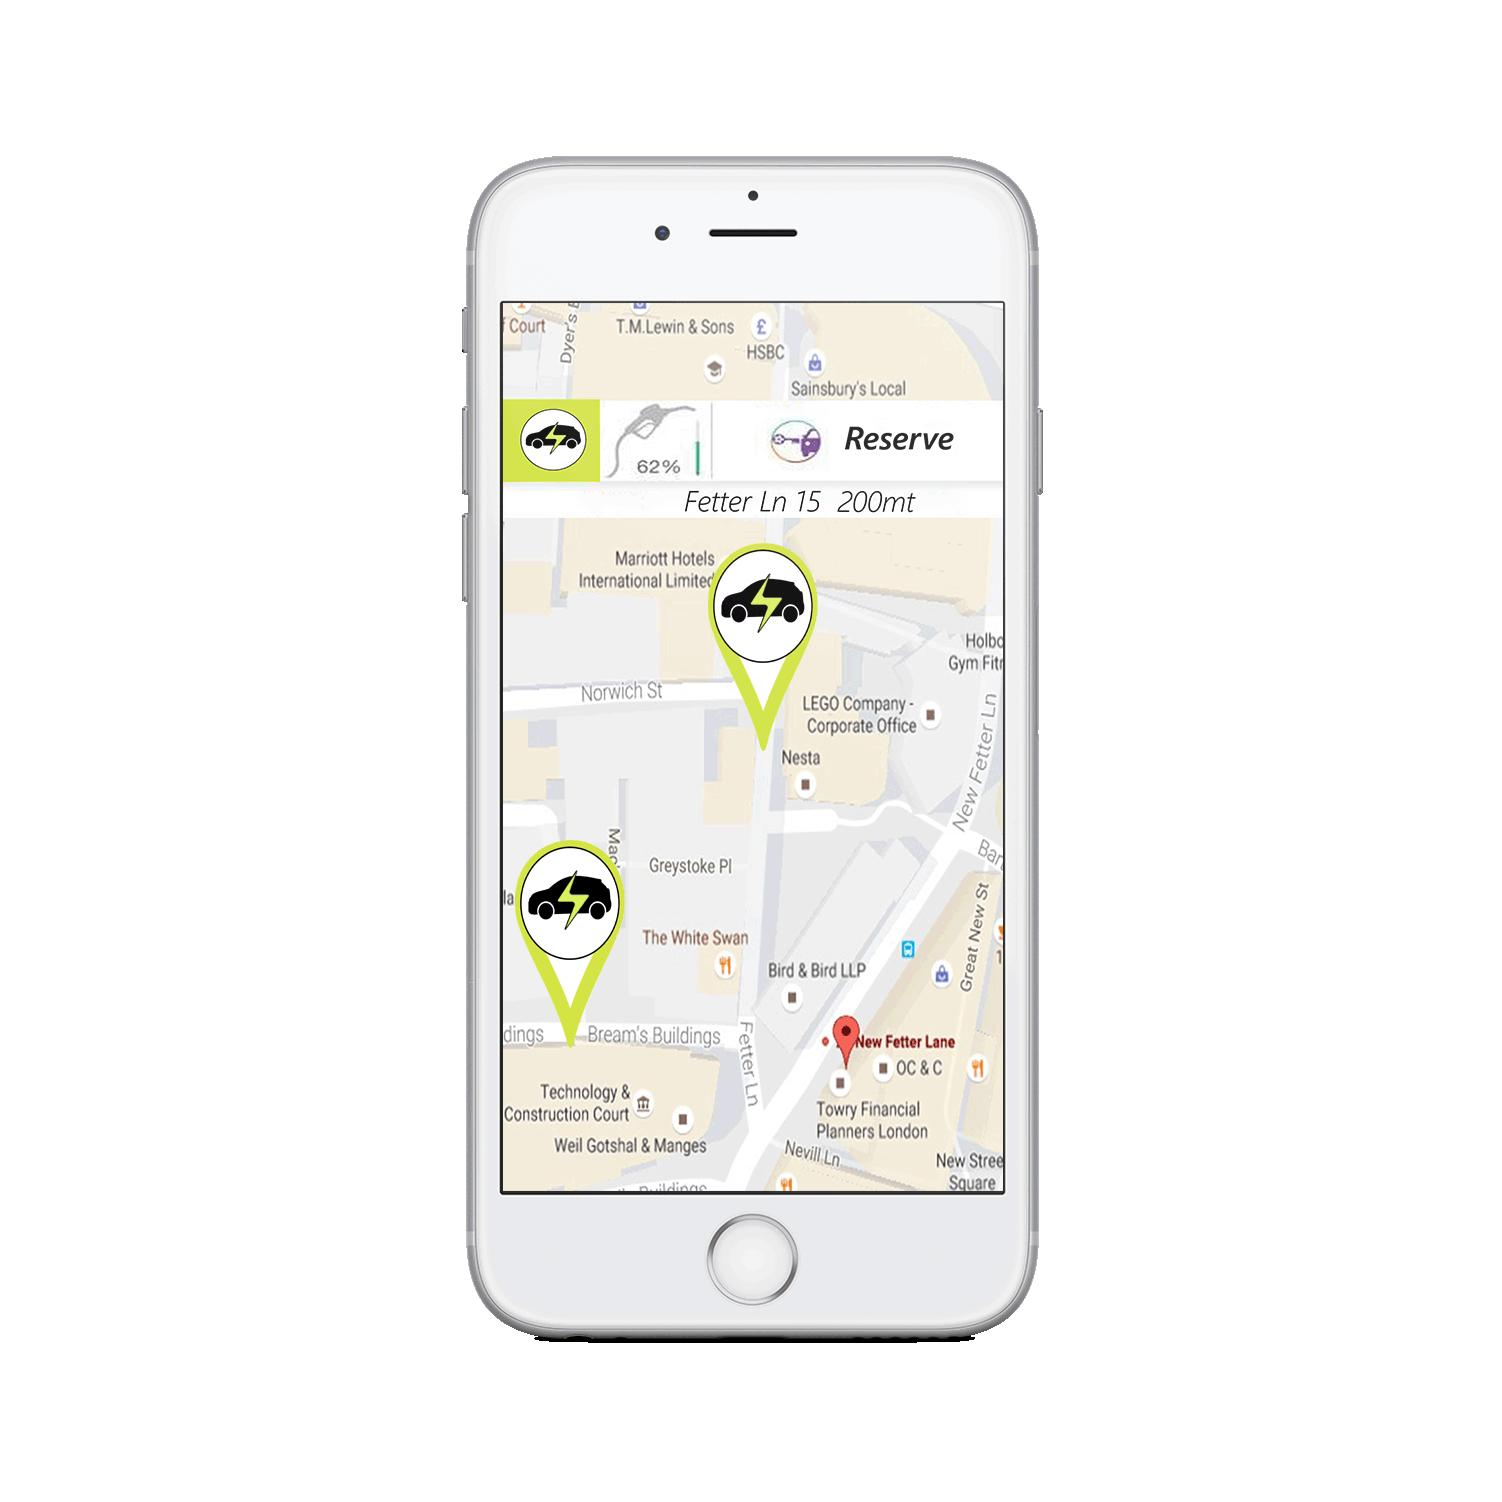
\includegraphics[width=400 pt]{resources/editato.jpg}
\caption{\label{fig:editato}View available car information in mobile application.}
\end{figure}

\subsubsection{View map on the website} This mockup shows the map that a generic user (guest or client) can see on the PowerEnJoy website.On the map are displayed the boundaries of the safe area in which a client can leave the car and the charging stations with the number of available charging spots.The user can insert an address in order to see the available cars within a certain distance.
\begin{figure}[h]
\centering
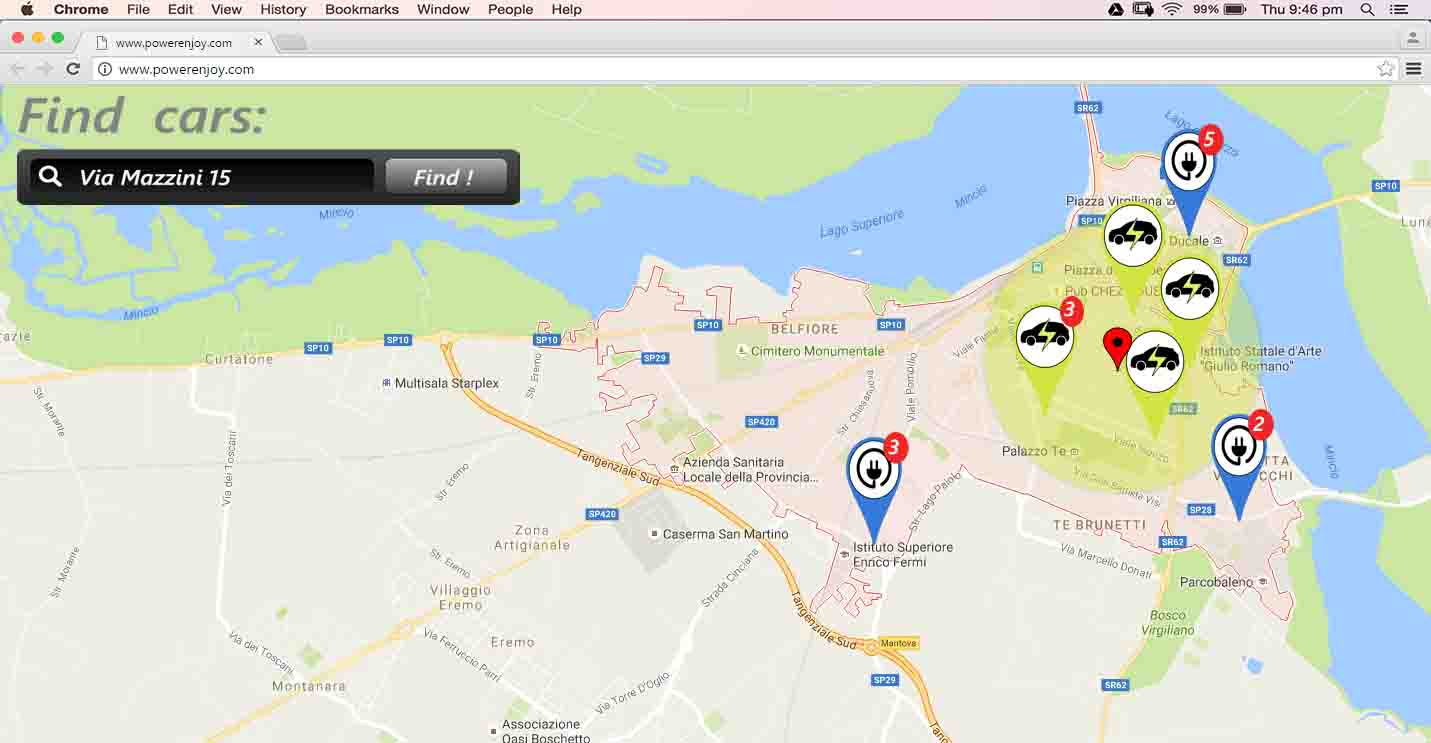
\includegraphics[width=450 pt]{resources/mappa.jpg}
\caption{\label{fig:mappa}View map on the website.}
\end{figure}

\subsubsection{Registration form} The mockup above shows the registration procedure that a guest has to complete in order to become a client and have access to the PowerEnJoy car sharing.

\begin{figure}[h]
\centering
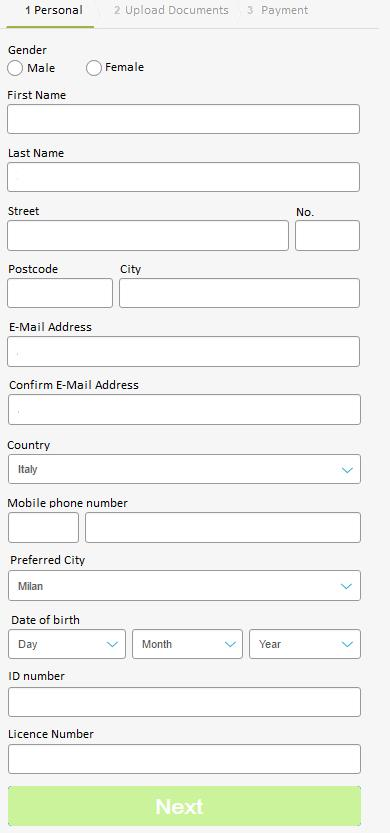
\includegraphics[height=200 pt]{resources/registrazione.jpg}
\caption{\label{fig:reg}Registration form.}
\end{figure}

\subsubsection{Insert pin on the car display} This mockup shows the form in which the client has to insert his pin. After inserting the correct pin the client can start the engine of the car.

\begin{figure}[ht]
\centering
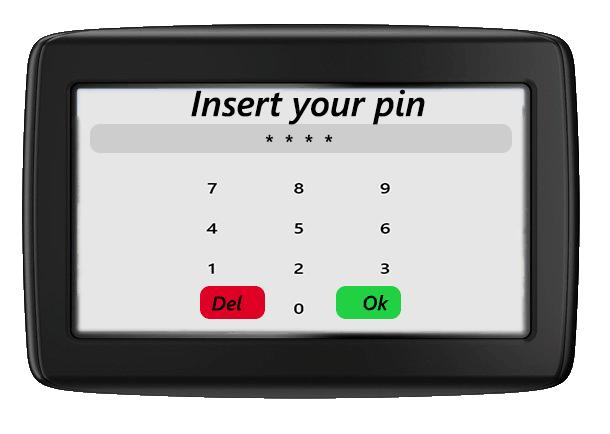
\includegraphics[width=400 pt]{resources/nav68.jpg}
\caption{\label{fig:pin}Insert pin on the car display.}
\end{figure}

\subsection{The world and the machine}

“The World and the Machine” model by M. Jackson and P. Zave is useful to identify the entities in the portion of system that has to be developed (\textbf{The Machine}) , the entities inside the portion of the real-world affected by the Machine (\textbf{The World}), and all  the \textbf{Shared Phenomena} that are controlled by the world and observed by the machine  or controlled by the machine and observed by the world.

\begin{figure}[ht]
\centering
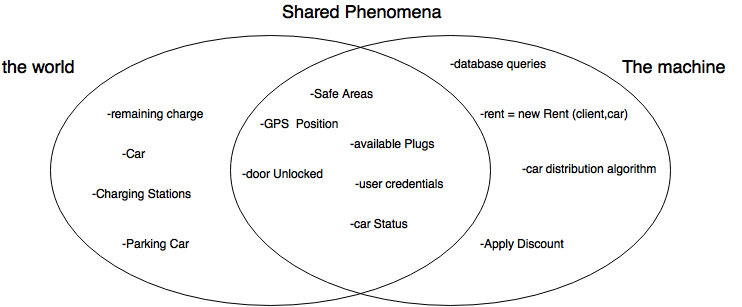
\includegraphics[width=400 pt]{resources/worldMachine.png}
\caption{\label{fig:WandM}The World and the Machine.}
\end{figure}


\newpage

\section{Scenarios}
%G1-registration
\subsection {Registration Scenario}
Alice heard from his friend Charles that there is a new eco-friendly car sharing service in her town and she wants to use it. She installs the application PowerEnJoy on her device, opens the registration section and compiles the form with her personal data, e-mail and a number of credit card. After she makes a photo of her driving license and ID-card and upload it. The system receives these information and verifies if they are valid making a request to the national transport's system. So, the system sends back to Alice her password, and allows her to rent a car. 

%G2-G3 - Log in and display car information
\subsection{Log in and display car information Scenario}
John has to make a long travel to a venue called 'The wall' and he finds out that the only reasonable way to get there is using a car sharing service. The only one he is yet registered is PowerEnJoy but he never used before and John does know nothing about that place. In order to plan his route he logs in the web application and see the available cars, the charging levels, the charging stations near his position and he discovers that 'The wall' is a safe area. 
%/ Denis : ho eliminato "a couple of hours before" perchè può confondere
%G4-reservation
\subsection{Reservation Scenario}
Bob needs to reach the airport at 3 am but there are no public transportation at that hour and the taxis are too expensive for him. So he decides to use the PowerEnJoy application from his his smartphone. Once found the closest available car on the map, he reserves it and starts moving to the car location." 
%Denis : "...his smartphone. Once found the closest available car on the map, he reserves it and starts moving to the car location."
%Claudio : ok. l'ho modificato


%G5-opening \rental G6 - display money charged 
\subsection{Opening / Rental scenario}
After 10 minutes of walk, Bob is in front of the car, he opens it using the app and he puts the luggage in the trunk. After identifying himself, he starts the engine and selects the destination. At this point the rent starts and Bob makes his way to the airport. 
While Bob is driving to the airport, he can check how much he is spending.
%/Denis : "Spending" è meno formale e più usato. ack 
%G7 ecology G8 
\subsection{Ecology Scenario}
Charles loves the PowerEnJoy philosophy of respecting nature and he uses the service every day to go work, there is a power station near his office so each time he parks the car there and plugs it into the power grid to get the discount. 
The office is located in a safe zone so whenever the power station is full he leaves the car in the near by, always checking that the system close the car before leaving.

%G9 - reporting abuse 
\subsection{Reporting abuse Scenario}
Hahn is a solo singer and he wants to make a walk in the park with his dog Chew and his child Loren. At the end of the day they are very tired and don't want to come back home walking so they decide to use PowerEnJoy, the system find that there is a car near by, in front of an ice-cream shop. When they arrive to the car Loren cannot resist to the temptation of the ice-cream so he starts crying and Hahn to makes him stops decides to buy him an ice-cream, but in the meanwhile Chew played in the mud because he was feeling alone. Hahn don't want to dirty the car but he sees that Jabba, a friend of him, is coming. Han have to pay Jabba a conspicuous amount of money and since that Hahn doesn't have that money yet he decides to jump in the car. Hahn is usual to drive very fast and near a semaphore he slam on the brakes and Loren drops the ice-cream, Chew jump to the front seat and eat it. Once they arrived they leave the car all dirty. After a while Anakin reserves the same car but he finds it dirty so he uses the service provided by the application and signals the abuse. PowerEnJoy applies a fee to Hahn and blocks the service to him for two month.
%/Denis : Deve essere più conciso, una persona che non ha mai visto Star Wars si annoia  e perde il filo del discorso.
%G10 - Saving Mode
\subsection{Saving Mode Scenario}
Donnie, Ester, Frank and Gabriela are students and they want to travel in the cheapest possible way. Today is Gabriela's birthday and they want to go to the mall to celebrate and since Gabriela is eco-friendly they decides to go with an electric car. Frank has a PowerEnJoy account so they decides to use the service and since they are cheap they use the money saving option. The application suggests them the nearest car with enough charge to reach the mall with a residual charge bigger than 50\%, then it gives direction to get to the car and once opened the terminal inside the car suggest the charging stations nearest to the mall, indicating them with different colors based on how many available plugs there are in each of them. Once they have chosen the charging station the system give directions. When they arrive  they plug the car in the charging grid and the system recognize that they are 4 people, that they plugged the car and that they left the car with more than 50\% of residual charge, so it applies 10\% + 30\% + 20\% of discount.
%\Denis : "Frank has a PowerEnJoy account and, in order to save money ,they decide to use the "money saving"  option" .  "When they arrive  they plug the car in the charging grid. The system recognize that they plugged the car , they left the car with more than 50\% of residual charge, and that there were 4 passengers, so it applies 10\% + 30\% + 20\% of discount. 
% Claudio : ok Denis, DIY"

\newpage

\section{UML models}
\subsection{Use Cases Description}
\subsubsection{Register to PowerEnJoy}
%
\textbf{Actors:}
Guest\\
%
\textbf{Entry Conditions:}
A guest enters in the registration section.\\ 
%
\textbf{Flow of events:}
\begin{enumerate}
\item The guest fills the form with his personal data, the number of his ID card and the number of the driving license. 
\item The guest uploads ID and driver license pictures.
\item  The guest fills the payment method form with his credit or prepaid card's information. 
\item PowerEnJoy verifies the correctness of the data and sends an email to the guest with his password and a pin necessary to start the rental. 
\item The guest confirms the registration throw the link and logs-in for the first time.
\item PowerEnJoy registers the guest as a new client. 
\end{enumerate}
%
\textbf{Exit Conditions:}
Guest successfully ends registration process and becomes a Client. From now on he can log in to the application using his credential and use the PowerEnJoy service. \\ 
%
\textbf{Exceptions:}
\begin{itemize}
\item If the guest inserts not valid data PowerEnJoy doesn't allow to complete the registration.
\item If the guest inserts and already used Email.
\\
\\In these 2 cases PowerEnJoy highlights the not valid fields and allows the guest to try again.
\item The system does not allow an existing user to register a second time.
\item If the Guest does not confirm his email within 48 hours PowerEnJoy cancels the request of registration and notifies that to the guest with an email.
\end{itemize}
%
\textbf{Special Requirements:}
\begin{itemize}
\item After the registration the client must be able to use the service after no longer than 5 minutes.
\item After that the user sends his document he must receive an email feedback with the confirmation link in no more than 10 minutes.
\item The communication of sensible data is made throw a protected channel.
\end{itemize}

%\Denis : 1. The visitor is already a user.  4. Email choosen is already associated to another user.



\subsubsection{Display a map information}
%
\textbf{Actors:}
User\\
%
\textbf{Entry Conditions:}
Entering in the map section. \\
%
\textbf{Flow of events:}
\begin{enumerate}
\item User sends his GPS position or selects an address on the map, and specifies a maximum distance from this point.
\item PowerEnJoy displays the data about the part of map requested: 
\begin{itemize}
\item location of available cars
\item location of charging areas and number of available charging spot
\item boundaries of safe areas 
\end{itemize}
\item User requests information about one selected car.
\item PowerEnJoy sends back the remaining charge percentage and the license plate number of the selected car .
\item User can see the requested information in a car information menu.
\end{enumerate}
%
\textbf{Exit Conditions:}
Exit from the map section, or a start of a reservation. \\
%
\textbf{Exceptions:}
\begin{itemize}
\item If User doesn't obtain a valid GPS signal, PowerEnJoy uses a default position like the center of city.
\item If User requests information about a car no more available, PowerEnJoy doesn't send any information about this, and all location of displayed cars are refreshed. 
\item If User selects an address out of city, PowerEnJoy uses a default position.
\end{itemize}
%
\textbf{Special Requirements:}
\begin{itemize}
\item The map will refresh every 10 seconds.
\end{itemize}


\subsubsection{Log-in}
%
\textbf{Actors:}
Client\\
%
\textbf{Entry Conditions:}
A client enters in the log-in section.\\
%
\textbf{Flow of events:}
\begin{enumerate}
\item The client enters his credentials.
\item PowerEnJoy verifies the correctness of the credentials.
\item PowerEnJoy redirects the client to the map section.
\end{enumerate}
%
\textbf{Exit Conditions:}
Client is logged in the system.\\
%
\textbf{Exceptions:}
\begin{itemize}
\item The client inserts not valid credentials.PowerEnJoy notifies him that an error and allows him to enter his email and password again.
\end{itemize}
%
\textbf{Special Requirements:}
\begin{itemize}
\item The system should provide a feedback in 10 seconds.
\end{itemize}


\subsubsection{Reserve a car}
%
\textbf{Actors:}
Logged Client\\
%
\textbf{Entry Conditions:}
A client clicks the Reserve button in the car information menu.\\
%
\textbf{Flow of events:}
\begin{enumerate}
\item PowerEnJoy sets the car as reserved.
\item The client receives the confirmation of the reservation.
\item The client checks the remaining time of the reservation.  
\end{enumerate}
%
\textbf{Exit Conditions:}
The car is no longer available, the client has now a rent in progress.\\
%
\textbf{Exceptions:}
\begin{itemize}
\item The client doesn't have the permission to reserve a car.
\item The client has yet canceled a reservation on the same car in the last 2 hours. 
\item The car is no longer available.
\end{itemize}
In all of these cases the reservation process is not performed and the user is redirected to the map section. \\
%
\textbf{Special Requirements:}
\begin{itemize}
\item The system should provide a feedback in 10 seconds.
\end{itemize}


\subsubsection{Open a car}
%
\textbf{Actors:}
Logged Client \\
%
\textbf{Entry Conditions:}
Client has done a reservation. \\
%
\textbf{Flow of events:}
\begin{enumerate}
\item Client moves to a car location, within an hour from the reservation.
\item Once he is arrived, he can push the open button from the application.
\item PowerEnJoy verifies if the client is  releases the block system of the car.
\item Client opens the car within a minute.
\end{enumerate}
%
\textbf{Exit Conditions:}
Client starts the rent. \\
%
\textbf{Exceptions:}
\begin{itemize}
\item If the client doesn't reach the car before one hour, PowerEnJoy deletes the reservation and applies a fee of 1 Euro.
\item If the client tries to open the car while he is far from the car or he has not GPS signal, PowerEnJoy doesn't unlock the car.
\end{itemize}
%
\textbf{Special Requirements:}
\begin{itemize}
\item PowerEnJoy unlocks the car within a minute from the request.
\end{itemize}



\subsubsection{Start the rent}
%
\textbf{Actors:}
Logged Client \\
%
\textbf{Entry Conditions:}
The system has opened the car.\\
%
\textbf{Flow of events:}
\begin{enumerate}
\item The Client inserts the pin.
\item The sistem after checking the correctness of the pin enables the possibility to turn on the engine.
\item The Client turns on the engine.
\item The Client selects his destination.
\item The car system shows the route and the current cost.
\item The Client starts moving to his destination.
\item The Client sees in real time how much he is spending.
\end{enumerate}
\textbf{Exit Conditions:}
The Client is driving the rented car.\\
%
\textbf{Exceptions:}
\begin{itemize}
\item If the charge of the car is lower then 15\% the car system signals to park the car immediately.
\item If the client continues driving until the car battery is empty the system applies a fee of 100 euros to the client.
\item If the rent takes more than 1 day the system signals the case to the operators system.
\end{itemize}
%
\textbf{Special Requirements:}
There are no special Requirements.



\subsubsection{End the rent}
%
\textbf{Actors:}
Logged Client \\
%
\textbf{Entry Conditions:}
Client reaches the destination. \\
%
\textbf{Flow of events:}
\begin{enumerate}
\item Client parks the car in a safe area and turn off the engine.
\item Client pushes the button for terminate the rent and exits from the car.
\item PowerEnJoy receives the request,checks if the car is parked in a safe area and, after one minute, locks the door of the car.
\item PowerEnJoy charges the client after 5 minutes to give the possibility to plug the car applying eventual discounts.
\end{enumerate}
%
\textbf{Exit Conditions:}
The car is set as available. \\
%
\textbf{Exceptions:}
\begin{itemize}
\item If the client tries to release the car out of a safe area, the system doesn't allow the end of rent.
\item If the client doesn't have enough money to pay the rent, PowerEnJoy disables the client account until the debt is absolved.
\item If the client doesn't exit from the car after one minute , the system doesn't lock the car doors and doesn't terminate the rent.
\end{itemize}
%
\textbf{Special Requirements:}
There are no special Requirements.



\subsubsection{Plug the car}
%
\textbf{Actors:}
Logged Client \\
%
\textbf{Entry Conditions:}
The Client parks the car in a charging station with free plugs and end the rent. \\
%
\textbf{Flow of events:}
\begin{enumerate}
\item The Client opens the charging slot of the car.
\item The Client plugs the plug to the car.
\item The car system applies a discount of 30\% to the last rent.
\end{enumerate}
%
\textbf{Exit Conditions:}
The car is correctly plugged - in and is recharging.\\
%
\textbf{Exceptions:}
If the client plugs the car after 5 minutes doesn't apply the discount\\
%
\textbf{Special Requirements:}
There are no Special Requirements.



\subsubsection{Report damaged/dirty car}
%
\textbf{Actors:}
Logged Client \\
%
\textbf{Entry Conditions:}
Client enters in a damaged or dirty car.\\
%
\textbf{Flow of events:}
\begin{enumerate}
\item A Client who notices that the car is damaged or dirty before starting the rent can report it by clicking the "Report damaged/dirty car" button.
\item PowerEnJoy redirects the client to a form where he has to indicate:
\begin{itemize}
\item Type of Abuse : "Damaged" or "Dirty" 
\item Gravity of the problem : from 0 to 5
\end{itemize}
\item PowerEnJoy signals the case to the operators system.
\item PowerEnJoy proposes to the client two alternatives :
\begin{itemize}
\item "Continue rent"
\item "End rent"
\end{itemize}
\item The client selects the desired choice.
\end{enumerate}
%
\textbf{Exit Conditions:}
The car is set unavailable.  \\
\textbf{Exceptions:}
 There are not exceptions. \\
\textbf{Special Requirements:}
 There are not Special Requirements\\

\subsubsection{Select money saving option}
%
\textbf{Actors:}
Logged Client \\
%
\textbf{Entry Conditions:}
The Client selects the save mode option in the car display\\
%
\textbf{Flow of events:}
\begin{enumerate}
\item The system estimates which is the most suitable charging station based on the city car distribution and the location chosen by the client. 
\item The car system suggests some possible charging stations.
\item The client selects one of the suggested charging stations.
\end{enumerate}
%
\textbf{Exit Conditions:}
The car system starts the navigation to the chosen charging station. \\
%
\textbf{Exceptions:}
\begin{itemize}
\item If the client doesn't like any of the suggested charging stations he can undo the action and proceed with the normal mode.
\end{itemize}
%
\textbf{Special Requirements:}
\begin{itemize}
\item The system should provide feedback within 10 seconds.
\end{itemize}


\newpage
\subsection{Use Case Diagram}

\begin{figure}[hp]
\centering
\includegraphics[width=400 pt]{resources/ucD.png}
\caption{\label{fig:ucD}Use Case Diagrams.}
\end{figure}

\newpage
\subsection{Class Diagram}

\begin{figure}[hp]
\centering
\includegraphics[width=430 pt]{resources/cD.png}
\caption{\label{fig:cD}Class Diagrams.}
\end{figure}

\newpage
\subsection{Sequence Diagrams}

\begin{figure}[hp]
\centering
\includegraphics[width=450 pt]{resources/sD1.png}
\caption{\label{fig:sD1}Reserve a car sequence diagram.}
\end{figure}

\begin{figure}[hp]
\centering
\includegraphics[width=450 pt]{resources/sD2.png}
\caption{\label{fig:sD2}Start the rent sequence diagram.}
\end{figure}

\begin{figure}[hp]
\centering
\includegraphics[width=450 pt]{resources/sD3.png}
\caption{\label{fig:sD3}End the rent sequence diagram.}
\end{figure}

\newpage

\section{Alloy}
\subsection{Code}
\lstinputlisting{resources/alloy.txt}

\subsection{Result}
This screenshot of the Alloy Analyzer software that shows the consistence of the model in all part.

\begin{figure}[h]
\centering
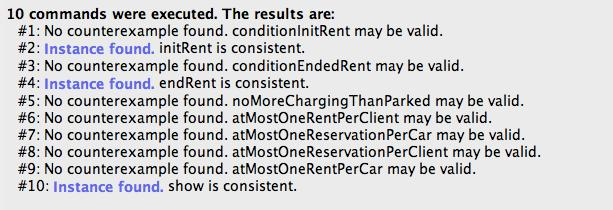
\includegraphics[width=450 pt]{resources/alloyResults.jpg}
\caption{\label{fig:AlloyRes}Alloy results.}
\end{figure}

\newpage
\subsection{Generated world}

\begin{figure}[hp]
\centering
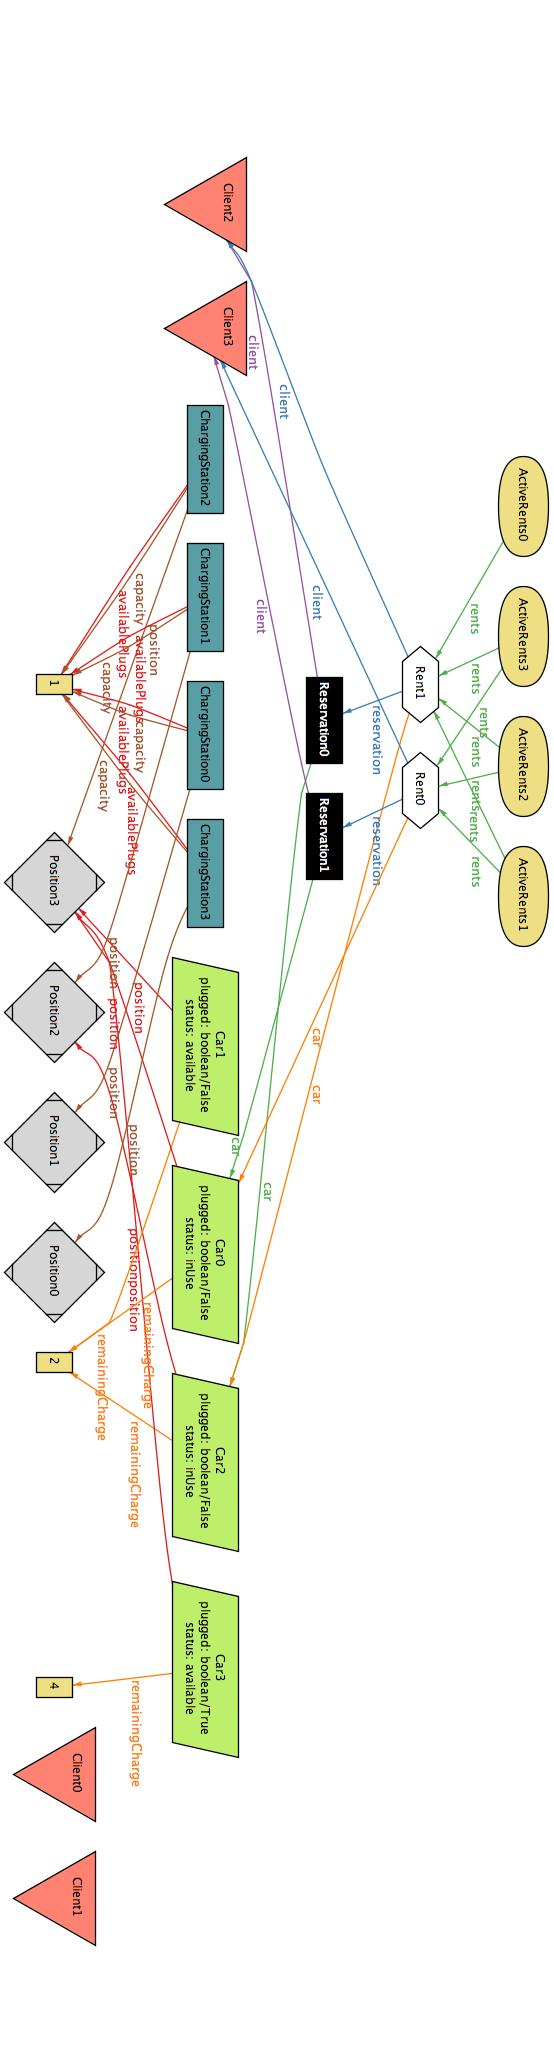
\includegraphics[height=526 pt]{resources/generatedWorld.jpg}
\caption{\label{fig:AlloyWorld}The world generated.}
\end{figure}

\newpage

\section{Appendix}
\subsection{Software and tool used}
The tools we used to create this RASD document are:
\begin{itemize}
\item Overleaf (for latex writing in parallel)
\item Photoshop (for mockups)
\item Draw.io (for UML diagrams)
\item Alloy
\end{itemize}

\subsection{Hours of work}
During the whole  project the team worked together each time with the following schedule:\\
\textbf{Claudio Salvatore Arcidiacono}
\begin{itemize}
\item 31 October : 16-20  4hours
\item 1 November : 15-21  6hours
\item 4 November : 14-21  7hours
\item 5 November : 16-20  4hours
\item 6 November : 14-20  6hours
\item 7 November : 17-22  5hours
\item 9 November : 18-21  3hours
\item 10 November : 18-21  3hours
\item 11 November : 11-22 (1hour of pause) 10hours
\item 12 November : 10-24  12hours (2hours of pause)
\item 13 November : 10-13 3 hours \\

\textbf{Total hours:} 60 hours.
\end{itemize}


\textbf{Antonio Di Bello}
\begin{itemize}
\item 31 October : 16-20  4hours
\item 1 November : 15-21  6hours
\item 4 November : 14-21  7hours
\item 5 November : 16-20  4hours
\item 6 November : 14-20  6hours
\item 7 November : 17-22  5hours
\item 9 November : 18-21  3hours
\item 10 November : 18-21  3hours
\item 11 November : 11-22 (1hour of pause) 10hours
\item 12 November : 10-24  12hours (2hours of pause)
\item 13 November : 10-13 3 hours \\

\textbf{Total hours:} 60 hours.
\end{itemize}


\textbf{Denis Dushi}
\begin{itemize}
\item 31 October : 16-20  4hours
\item 1 November : 15-21  6hours
\item 4 November : 14-21  7hours
\item 5 November : 16-20  4hours
\item 6 November : 14-20  6hours
\item 7 November : 17-22  5hours
\item 9 November : 18-21  3hours
\item 10 November : 18-21  3hours
\item 11 November : 11-22 (1hour of pause) 10hours
\item 12 November : 10-24  12hours (2hours of pause)
\item 13 November : 10-13 3 hours \\

\textbf{Total hours:} 60 hours.
\end{itemize}
\subsection{Changelog}

\end{document}